\section{A Brief Description of Autograd}
As part of a modern deep learning framework, we need to define functional units like 
the one shown in \autoref{fig:ch2:block_form}. In particular, not only must we
be able to calculate the forward evaluation of a block $y=f(x,w)$ given an input $x$ and 
(possibly) some learnable weights $w$, we must also be able to
calculate the passthrough and update gradients $\dLdx{x}$, $\dLdx{w}$. This
typically involves saving $\dydx{y}{x}$ and $\dydx{y}{w}$ evaluated at the current
values of $x$ and $w$ when we calculate the forward pass. 

For example, the simple ReLU $y = \F{max}(0,\ x)$ is not memory-less. On the
forward pass, we need to put a 1 in all the positions where $x > 0$, and a 0
elsewhere. Similarly for a convolutional layer, we need to save $x$ and $w$ to
correlate with $\dLdx{y}$ on the backwards pass. It is up to the block designer
to manually calculate the gradients and design the most efficient way of
programming them.

For clarity and repeatability, we give pseudocode for all the core operations
developed in our package \emph{PyTorch Wavelets}. We carry this through to other chapters
when we design different wavelet based blocks. By the end of this thesis, it should be
clear how every attempted method has been implemented.

% Using inbuit blocks is very useful and makes development and testing quick to
% do. However, when doing operations with fixed filters such as those found in
% wavelet transforms, autograd will unnecessarily save lots of activations, using
% precious GPU memory. This is why as part of this thesis we describe how 
% autograd blocks units for the operations we use/have developed.

Note that the pseudo code can be one of three types of functions:
\begin{enumerate}
  \item Gradient-less code - these are low-level functions that can be used for
    both the forward and backward calculations. E.g. \autoref{alg:ch3:fb1d}. We
    name these \texttt{NG:<name>}, NG for no gradients.
  \item Autograd blocks - the modules as shown in
    \autoref{fig:ch2:block_form}. These always have a forward and backward pass, and 
    are named \texttt{AG:<name>}. E.g. \autoref{alg:ch3:dwt}.
  \item Higher level modules - these make use of efficient autograd functions
    and are named \texttt{MOD:<name>}. E.g. \autoref{alg:ch3:dtcwt}.
\end{enumerate}

% \begin{figure}
  % \centering
  % \begin{tikzpicture}[every node/.style={node font=\large}]
\definecolor{mycolor}{RGB}{252,247,189};
\pgfmathsetmacro{\EDGE}{.5}
\node [fill=mycolor, draw, minimum width=3cm, minimum height=2cm] (block) at (1,1) {$y=f(x,w)$};
\coordinate[right=\EDGE of block.south west] (xin);
\coordinate[left=\EDGE of block.south east] (dxin);
\coordinate[below=\EDGE of block.north west] (win);
\coordinate[above=\EDGE of block.south west] (dwin);
\coordinate[right=\EDGE of block.north west] (yin);
\coordinate[left=\EDGE of block.north east] (dyin);
\draw[<-] (xin) -- +(0,-1) node[below] {$x$};
\draw[->] (dxin) -- ++(0,-1) node[below] {$\dydx{\logloss}{x}$};
\draw[<-] (win) -- ++(-1,0) node[left] {$w$};
\draw[->] (dwin) -- ++(-1,0) node[left] {$\dydx{\logloss}{w}$};
\draw[->] (yin) -- ++(0,1) node[above] {$y$};
\draw[<-] (dyin) -- ++(0,1) node[above] {$\dydx{\logloss}{y}$};
\end{tikzpicture}

  % \mycaption{An autograd block}{The building block of modern deep learning
  % frameworks. Every function needs to be able to not only take an input (and
  % possibly a weight parameter) to give an output $y=f(x,w)$, it must also 
  % be able to take a backpropagated input $\dLdx{y}$ and give
  % backpropagated outputs $\dLdx{x},\ \dLdx{w}$. The
  % former is then passed onto the previous block's backpropagated input, and the
  % latter, if it exists, is used to update weights. As a key step in 
  % doing this, the gradients $\dydx{y}{x},\ \dydx{y}{w}$ evaluated at the current
  % values of $x$ and $w$ must be saved on the forward pass. This takes up memory
  % which can then be freed once the backpropagated outputs have been calculated.}
  % \label{fig:ch3:autograd_blk}
% \end{figure}

\section{Fast Calculation of the DWT and IDWT}\label{sec:ch3:dwt}
\begin{figure}
  \centering
  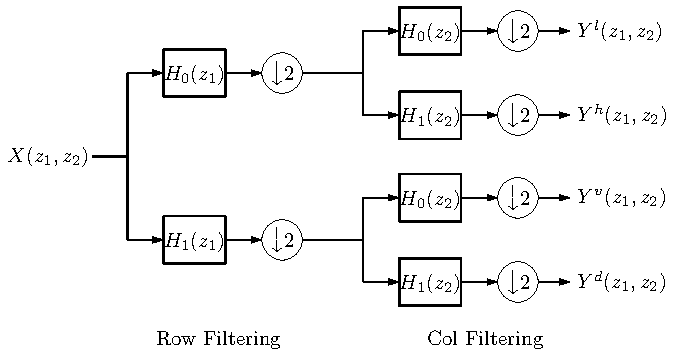
\includegraphics[width=0.8\textwidth]{\imgpath/dwt2d.pdf}
  \mycaption{Block Diagram of 2-D DWT}{The components of a filter bank DWT in
  two dimensions. $Y^l, Y^h, Y^v, Y^d$ represent the lowpass, horizontal,
  vertical, and diagonal components.}
  \label{fig:ch3:dwt}
\end{figure}

To have a fast implementation of the Scattering Transform, we need a fast
implementation of the $\DTCWT$. For a fast implementation of the $\DTCWT$ we
need a fast implementation of the DWT. Future work may also explore
the DWT as a basis for learning, so having an implementation that is fast and
can pass gradients through will prove beneficial in and of itself.

There has been much research into the best way to do the DWT on a GPU, in
particular comparing the speed of Lifting \cite{sweldens_lifting_1998}, or second
generation wavelets, to the direct convolutional methods.
\cite{tenllado_parallel_2008, galiano_improving_2011} are two notable such
publications, both of which find that the convolution based implemetations are
better suited for the massively parallel architecture found in modern GPUs. For
this reason, we implement a convolutional based DWT.

Writing a DWT in low-level calls is not theoretically difficult to do.
There are only a few things to be wary of. Firstly, a `convolution' in most deep
learning packages is in fact a correlation. This does not make any difference
when learning but when using preset filters, as we want to do, it means that we
must take care to reverse the filters beforehand. Secondly, the automatic 
differentiation will naturally save activations after every step in the DWT
(e.g. after row filtering, downsampling and column filtering). This is for the
calculation of the backwards pass. We do not need to save these intermediate
activations and we can save a lot of memory by overwriting the automatic
differentiation logic and defining our own backwards pass.

\subsection{Primitives}\label{sec:ch3:primitives}
We start with the commonly known property that for a convolutional block, the
gradient with respect to the input is the gradient with respect to the output
convolved with the time reverse of the filter. More formally, if 
$Y(z) = H(z) X(z)$:
%
\begin{equation}\label{eq:ch3:backprop}
  \Delta X(z) = H(z^{-1}) \Delta Y(z)
\end{equation}
%
where $H(z^{-1})$ is the $Z$-transform of the time/space reverse of $H(z)$,
$\Delta Y(z) \triangleq \dydx{L}{Y}(z)$ is the gradient of the loss with respect
to the output, and $\Delta X(z) \triangleq \dydx{L}{X}(z)$ is the gradient of
the loss with respect to the input. This was proved in \autoref{sec:ch2:conv_grad}, we 
have just rewritten it in terms of $Z$-transforms here.

Additionally, if we decimate by a factor of two on the forwards pass, the
equivalent backwards pass is interpolating by a factor of two (see \autoref{sec:app:samplegrads}
for a proof of this).

\autoref{fig:ch3:dwt} shows the block diagram for performing the forward pass of
a DWT. 
Like Matlab, most deep learning frameworks have an efficient function for
doing convolution followed by downsampling. Similarly, there is an efficient
function to do upsampling followed by convolution (for the inverse transform).
Using the above two properties for the backwards pass of convolution and sample
rate changes, we quickly see that the backwards pass of a wavelet transform is
simply the inverse wavelet transform with the time reverse of the analysis
filters used as the synthesis filters. For orthogonal wavelet transforms, the
synthesis filters are the time reverse of the analysis filters so
backpropagation can simply be done by calling the inverse wavelet transform on
the wavelet coefficient gradients. See \autoref{sec:app:analysis_gradient} for a
proof of this.

\subsection{The Forward and Backward Algorithms}
Let us start by giving generic names to the above mentioned primitives. We call
a convolution followed by downsample \texttt{conv2d_down}\footnote{E.g.\ In
PyTorch, convolution followed by downsampling is done with a call to
\texttt{torch.nn.functional.conv2d} with the stride parameter set to 2}. As
mentioned earlier, in all deep learning packages, this function's name is misleading as
it in fact does correlation. As such we need to be careful to reverse the
filters with \texttt{flip} before calling it. We call convolution followed by
upsampling \texttt{conv2d_up}\footnote{Similarly, this is done with 
\texttt{torch.nn.functional.conv_transpose2d} with the stride parameter set to
2 in PyTorch}. Confusingly, this function does in fact do true convolution, so
we do not need to reverse any filters. 

These functions in turn call the cuDNN low-level fucntions which can only support
zero padding. If another padding type is desired, it must be done beforehand
with a padding function \texttt{pad}.

\subsubsection{The Input}
In all the work in the following chapters, we would like to work on four
dimensional arrays. The first dimension represents a minibatch of $N$ images;
the second is the number of channels $C$ each image has. For a colour image,
$C=3$, but this often grows deeper in the network. Finally, the last two
dimensions are the spatial dimensions, of size $H\x W$. 

\subsubsection{1-D Filter Banks}
Let us assume that the analysis ($h_0,\ h_1$) and synthesis ($g_0,\ g_1$)
filters are already in the form needed to do column filtering. The necessary
steps to do the 1-D analysis and synthesis are described in
\autoref{alg:ch3:fb1d}. We do not need to define backpropagation functions for the
\texttt{afb1d} and \texttt{sfb1d} functions as they are each others backwards
step.

\begin{algorithm}[tb]
\caption{1-D analysis and synthesis stages of a DWT}\label{alg:ch3:fb1d}
\begin{algorithmic}[1]
\Function{NG:afb1d}{$x,\ h_0,\ h_1,\ mode,\ axis$}
  % \mbox{\\$h_0,\ h_1$ are 1-D lowpass and highpass filters}
  \State $ h_0,\ h_1 \gets \F{flip}(h_0),\ \F{flip}(h_1) $\Comment{flip the filters for \texttt{conv2d_down}}
  \If{axis == -1} 
    \State $h_0,\ h_1 \gets h_0^t,\ h_1^t$  \Comment{row filtering}
  \EndIf
  \State $p \gets \lfloor (\F{len}(x) + \F{len}(h_0) - 1) / 2 \rfloor$ \Comment{calculate output size}
  \State $b \gets \lfloor p/2 \rfloor$ \Comment{calculate pad size before}
  \State $a \gets \lceil p/2 \rceil$ \Comment{calculate pad size after}
  \State $x \gets \F{pad}(x,\ b,\ a,\ mode)$ \Comment{pre pad the signal with selected mode} 
  \State $lo \gets \mathtt{conv2d\_down} (x, h_0)$
  \State $hi \gets \mathtt{conv2d\_down} (x, h_1)$
  \State \textbf{return} $lo,\ hi$
\EndFunction
\end{algorithmic}\vspace{10pt}
\begin{algorithmic}[1]
\Function{NG:sfb1d}{$lo,\ hi,\ g_0,\ g_1,\ mode,\ axis$}
  % \mbox{\\$g_0,\ g_1$ are 1-D lowpass and highpass filters.}
  \If{axis == -1} 
    \State $g_0,\ g_1 \gets g_0^t,\ g_1^t$  \Comment{row filtering}
  \EndIf
  \State $p \gets \F{len}(g_0) - 2$ \Comment{calculate output size}
  \State $lo \gets \F{pad}(lo,\ p,\ p,\ ``zero")$ \Comment{pre pad the signal with zeros} 
  \State $hi \gets \F{pad}(hi,\ p,\ p,\ ``zero")$ \Comment{pre pad the signal with zeros} 
  \State $x \gets \mathtt{conv2d\_up}(lo,\ g_0) + \mathtt{conv2d\_up}(hi,\ g_1)$
  \State \textbf{return} $x$
\EndFunction
\end{algorithmic}
\end{algorithm}

\subsubsection{2-D Transforms and their gradients}
Having built the 1-D filter banks, we can easily generalize this to 2-D.
Furthermore we can now define the backwards steps of both the forward DWT
and the inverse DWT using these filter banks. We show how to do do this in 
\autoref{alg:ch3:dwt}. Note that we have allowed for different row and column
filters in \autoref{alg:ch3:dwt}. Most commonly used wavelets will use the same 
filter for both directions (e.g.\ the orthogonal Daubechies family), but later
when we use the $\DTCWT$, we will want to have different horizontal and vertical
filters.

The inverse transform logic is moved to the appendix
\autoref{alg:ch3:idwt}. An interesting result is the similarity between the two 
transforms' forward and backward stages. Further, note that the only things that
need to be saved are the filters, as seen in
Algorithm~\algref{alg:ch3:dwt}{line:ch3:dwt_save}. These are typically only a
few floats, giving us a large saving over relying on autograd.

A multiscale DWT (and IDWT) can easily be made by calling \autoref{alg:ch3:dwt}
(\autoref{alg:ch3:idwt}) multiple times on the lowpass output (reconstructed
image). Again, no intermediate activations need be saved, giving this
implementation almost no memory overhead. 

\begin{algorithm}[tb]
\caption{2-D DWT and its gradient}\label{alg:ch3:dwt}
\begin{algorithmic}[1]
\Function{AG:DWT:FWD}{$x,\ h_0^c,\ h_1^c,\ h_0^r, h_1^r,\ mode$}
  \State \textbf{save} $h_0^c,\ h_1^c,\ h_0^r,\ h_1^r,\ mode$ \Comment{For the backwards pass} \label{line:ch3:dwt_save}
  % \State $lo,\ hi \gets \F{afb1d}(x,\ h_0^c,\ h_1^c,\ mode,\ axis=-2)$ \Comment{column filter}
  % \State $ll,\ lh \gets \F{afb1d}(lo,\ h_0^r,\ h_1^r,\ mode,\ axis=-1)$ \Comment{row filter}
  % \State $hl,\ hh \gets \F{afb1d}(hi,\ h_0^r,\ h_1^r,\ mode,\ axis=-1)$ \Comment{row filter}
  \State $lo,\ hi \gets \F{afb1d}(x,\ h_0^r,\ h_1^r,\ mode,\ axis=-1)$ \Comment{row filter}
  \State $ll,\ lh \gets \F{afb1d}(lo,\ h_0^c,\ h_1^c,\ mode,\ axis=-1)$ \Comment{column filter}
  \State $hl,\ hh \gets \F{afb1d}(hi,\ h_0^c,\ h_1^c,\ mode,\ axis=-1)$ \Comment{column filter}
  \State \textbf{return} $ll,\ lh,\ hl,\ hh$
\EndFunction
\end{algorithmic}\vspace{10pt}
\begin{algorithmic}[1]
\Function{AG:DWT:BWD}{$\Delta ll,\ \Delta lh,\ \Delta hl,\ \Delta hh$}
  \State \textbf{load} $h_0^c,\ h_1^c,\ h_0^r,\ h_1^r,\ mode$
  \State $ h_0^c,\ h_1^c \gets \F{flip}(h_0^c),\ \F{flip}(h_1^c) $\Comment{flip the filters as in \eqref{eq:ch3:backprop}}
  \State $ h_0^r,\ h_1^r \gets \F{flip}(h_0^r),\ \F{flip}(h_1^r)$ 
  % \mbox{\\$g_0,\ g_1$ are 1-D lowpass and highpass filters.}
  \State $\Delta lo \gets \F{sfb1d}(\Delta ll,\ \Delta lh,\ h_0^c,\ h_1^c,\ mode,\ axis=-2) $
  \State $\Delta hi \gets \F{sfb1d}(\Delta hl,\ \Delta hh,\ h_0^c,\ h_1^c,\ mode,\ axis=-2) $
  \State $\Delta x \gets \F{sfb1d}(\Delta lo,\ \Delta hi,\ h_0^r,\ h_1^r,\ mode,\ axis=-1) $
  \State \textbf{return} $\Delta x$
\EndFunction
\end{algorithmic}
\end{algorithm}


\section{Fast Calculation of the $\DTCWT$}\label{sec:ch3:dtcwt}
We have built upon previous implementations of the $\DTCWT$, in particular
\cite{kingsbury_dtcwt_2003, cai_2-d_2011, wareham_dtcwt_2014}. The $\DTCWT$ gets
is name from having two sets of filters, $a$ and $b$. In two dimensions, we do
four multiscale DWTs, called $aa$, $ab$, $ba$ and $bb$, where the pair of letters indicates
which set of wavelets is used for the row and column filtering. The twelve
bandpass coefficients at each scale are added and subtracted from each other to
get the six orientations' real and imaginary components \autoref{alg:ch3:q2c}.
The four lowpass coefficients from each scale can be used for the next scale
DWTs. At the final scale, they can be interleaved to get four times the expected
decimated lowpass output area.

A requirement of the $\DTCWT$ is the need to use different filters for the first
scale to all subsequent scales \cite{selesnick_dual-tree_2005}. We have not
shown this in \autoref{alg:ch3:dtcwt} for simplicity, but it would simply mean
we would have to handle the $j=0$ case separately.

\begin{algorithm}[tb]
\caption{2-D $\DTCWT$}\label{alg:ch3:dtcwt}
\begin{algorithmic}[1]
\Function{MOD:DTCWT}{$x,\ J,\ mode$}
\State \textbf{load} $h_0^a,\ h_1^a,\ h_0^b,\ h_1^b$
\State $ll^{aa},\ ll^{ab},\ ll^{ba},\ ll^{bb} \gets x$
% \State $H = \left[h_
\For{$0 \le j < J$}
  \State $ll^{aa},\ lh^{aa},\ hl^{aa},\ hh^{aa} \gets \F{AG:DWT}(ll^{aa},\ h_0^a,\ h_1^a,\ h_0^a,\ h_1^a,\ mode)$
  \State $ll^{ab},\ lh^{ab},\ hl^{ab},\ hh^{ab} \gets \F{AG:DWT}(ll^{ab},\ h_0^a,\ h_1^a,\ h_0^b,\ h_1^b,\ mode)$
  \State $ll^{ba},\ lh^{ba},\ hl^{ba},\ hh^{ba} \gets \F{AG:DWT}(ll^{ba},\ h_0^b,\ h_1^b,\ h_0^a,\ h_1^a,\ mode)$
  \State $ll^{bb},\ lh^{bb},\ hl^{bb},\ hh^{bb} \gets \F{AG:DWT}(ll^{bb},\ h_0^b,\ h_1^b,\ h_0^b,\ h_1^b,\ mode)$
  \State \begin{varwidth}[t]{\linewidth}
    $yh[j] \gets \F{Q2C}( $\par 
        \hskip\algorithmicindent $lh^{aa},\ hl^{aa},\ hh^{aa},$ \par
        \hskip\algorithmicindent $lh^{ab},\ hl^{ab},\ hh^{ab},$ \par
        \hskip\algorithmicindent $lh^{ba},\ hl^{ba},\ hh^{ba},$ \par
        \hskip\algorithmicindent $lh^{bb},\ hl^{bb},\ hh^{bb})$
        \end{varwidth}
\EndFor
\State $yl \gets \F{interleave}(ll^{aa},\ ll^{ab},\ ll^{ba},\ ll^{bb})$
\State \textbf{return} $yl,\ yh$
\EndFunction
\end{algorithmic}\vspace{10pt}
\end{algorithm}

\section{Changing the ScatterNet Core}\label{sec:ch3:scat}
Now that we have a forward and backward pass for the $\DTCWT$, the final missing
piece is the magnitude operation. Again, it is not difficult to calculate the
gradients given the direct form, but we must be careful about their size. If $z
= x + jy$, then:
%
\begin{equation}
  r = |z| =  \sqrt{x^2 + y^2}
\end{equation}
%
This has two partial derivatives, $\dydx{r}{x},\ \dydx{r}{y}$:
\begin{align}
  \dydx{r}{x} & =  \frac{x}{\sqrt{x^2 + y^2}} = \frac{x}{r}\\
  \dydx{r}{y} & =  \frac{y}{\sqrt{x^2 + y^2}} = \frac{y}{r} 
\end{align}
Given an input gradient, $\Delta r$, the passthrough gradient is:
\begin{eqnarray}
  \Delta z & = & \Delta r \dydx{r}{x} + j\Delta r \dydx{r}{y} \\
           &= & \Delta r \frac{x}{r} + j\Delta r \frac{y}{r} \\
           &=& \Delta r e^{j\theta}
\end{eqnarray}
where $\theta = \arctan{\frac{y}{x}}$. This has a nice interpretation to it as
well, as the backwards pass is simply reinserting the discarded phase
information. The pseudo-code for this operation is shown in
\autoref{alg:ch3:mag}.
%

These partial derivatives are restricted to be in the range $[-1, 1]$ but have a singularity at the origin. 
In particular:
\begin{align}
  \lim_{x\rightarrow 0^{-},y\rightarrow 0}  \dydx{r}{x} &= -1 \\
  \lim_{x\rightarrow 0^{+},y\rightarrow 0}  \dydx{r}{x} &= +1 \\
  \lim_{x\rightarrow 0,y\rightarrow 0^{-}}  \dydx{r}{y} &= -1 \\
  \lim_{x\rightarrow 0,y\rightarrow 0^{+}}  \dydx{r}{y} &= +1 
\end{align}
These partial derivatives are very rapidly varying around 0 and the second
derivatives go to infinity at the origin. This is not a
feature commonly seen with other nonlinearities such as the tanh and sigmoid
but it is seen with the ReLU. Small changes in the input can cause large changes
in the propagated gradients.
The bounded nature of the first derivative somewhat restricts the impact of
possible problems so
long as our optimizer does not use higher order derivatives (this is commonly
the case). Nonetheless, we propose to slightly smooth the magnitude operator:

\begin{equation}\label{eq:ch3:magbias}
 r_s = \sqrt{x^2 + y^2 + b^2} - b
\end{equation}

This keeps the magnitude near zero for small $x,y$ but does slightly shrink larger
values. The gain we get however is a new smoother gradient surface.
% \textbf{Plot this}
We can then choose the size of $b$ as a hyperparameter in
optimization. The partial derivatives now become:
\begin{eqnarray}
  \dydx{r_s}{x} & = & \frac{x}{\sqrt{x^2 + y^2+b^2}} = \frac{x}{r_s}\\
  \dydx{r_s}{y} & = & \frac{y}{\sqrt{x^2 + y^2+b^2}} = \frac{y}{r_s} 
\end{eqnarray}
There is a memory cost associated with this, as we will now need to save both
$\dydx{r_s}{x}$ and $\dydx{r_s}{y}$ as opposed to saving only the phase.
\autoref{alg:ch3:mag_smooth} has the pseudo-code for this.

\begin{algorithm}[tb]
\caption{Magnitude forward and backward steps}\label{alg:ch3:mag}
\begin{algorithmic}[1]
\Function{AG:MAG:FWD}{$x,\ y$}
  \State $r \gets \sqrt{x^2 + y^2}$
  \State $\theta \gets \arctan2(y,\ x)$ \Comment{$\arctan2$ handles $x=0$}
  \State \textbf{save} $\theta$ 
  \State \textbf{return} $r$
\EndFunction
\end{algorithmic}\vspace{10pt}
\begin{algorithmic}[1]
\Function{AG:MAG:BWD}{$\Delta r$}
  \State \textbf{load} $\theta$
  \State $\Delta x \gets \Delta r \cos{\theta}$ \Comment{Reinsert phase}
  \State $\Delta y \gets \Delta r \sin{\theta}$ \Comment{Reinsert phase}
  \State \textbf{return} $\Delta x,\ \Delta y$
\EndFunction
\end{algorithmic}
\end{algorithm}

Now that we have the $\DTCWT$ and the magnitude operation, it is straightforward
to get a $\DTCWT$ scattering layer, shown in \autoref{alg:ch3:dtcwt_scat}. To
get a multilayer scatternet, we can call the same function again on $Z$, which
would give $S_0,\ S_1$ and $U_2$ and so on for higher orders. 

Note that for ease in handling the different sample rates of the lowpass and the
bandpass, we have averaged the lowpass over a $2\x 2$ window and downsampled it
by 2 in each direction. This slightly
affects the higher order coefficients, as the true $\DTCWT$ needs the doubly
sampled lowpass for the second scale. We noticed little difference in
performance from doing the true $\DTCWT$ and the decimated one.

\begin{algorithm}[tb]
  \mycaption{$\DTCWT$ ScatterNet Layer}{High level block using the above
  autograd functions to calculate a first order scattering}\label{alg:ch3:dtcwt_scat}
\begin{algorithmic}[1]
\Function{MOD:DTCWT\_SCAT}{$x,\ J=2,\ M=2$}
\State $Z \gets x$
\For{$0 \le m < M$}
  \State $yl,\ yh \gets \DTCWT(Z,\ J=1,\ mode=\F{`symmetric'})$
  \State $S \gets \F{avg\_pool}(yl,\ 2)$
  \State $U \gets \F{mag}(\real{yh},\ \imag{yh})$ 
  \State $Z \gets \F{concatenate}(S,\ U,\ axis=1)$ \Comment{stack 1 lowpass with 6 magnitudes}
\EndFor
\If{$J > M$}
\State $Z \gets \F{avg\_pool}(Z,\ 2^{J-M})$
\EndIf
\State \textbf{return} $Z$
\EndFunction
\end{algorithmic}
\end{algorithm}
